\documentclass[12pt,a4paper]{article}
\usepackage[utf8]{inputenc}
\usepackage[T1]{fontenc}
\usepackage{lmodern}
\usepackage{microtype}
\setlength{\emergencystretch}{2em}
\usepackage{amsmath,amssymb}
\usepackage{geometry}
\geometry{margin=2.5cm}
\usepackage{graphicx}
\usepackage{booktabs}
\usepackage{float}
\usepackage{xcolor}
\usepackage{caption}
\usepackage{enumitem}
\usepackage[authoryear,round]{natbib}
\usepackage{hyperref}
\hypersetup{colorlinks=true, linkcolor=black, citecolor=black, urlcolor=blue}


\newcommand{\corr}[1]{#1}
\newenvironment{correction}{}{}

\title{\textbf{Modeling Tail Dependence and Optimizing Multi-Asset Portfolios}\\[1em]
\large A Vine Copula Approach}
\author{\Large Ricardo DONTE}
\date{January 16, 2026\\[0.3em]Revised October 2026\\[5em]
\textit{UM6P-Africa Business School}\\
Master in Financial Engineering}

\begin{document}
\maketitle
\thispagestyle{empty}
\begin{center}\small The original report was written in French and translated into English by ChatGPT.\end{center}
\vfill

\newpage

\tableofcontents
\newpage

% =====================================================================================================
\section{Introduction}
\subsection{Motivation and Research Question}

New asset classes and recurring systemic crises have exposed limitations in conventional portfolio risk management. Classical allocation methods derived from Markowitz's mean--variance framework use linear correlations to describe dependence. A Gaussian model can understate the risk of joint extremes, particularly when diversification matters most.

During market stress, assets that normally offer diversification can fall together as asymmetric dependencies emerge. Linear correlation gives limited information about such tail events and can overstate the benefits of diversification. This study examines how to model extreme dependence across financial assets.

\subsection{Objectives and Methodology}

We combine ARMA-GARCH models with vine copulas, following an approach similar to \cite{evkaya2024}. The pair-copula construction separates each asset's marginal dynamics from their joint dependence and allows us to study joint crashes. We first estimate tail dependence across four asset classes, including Bitcoin. We then evaluate allocation strategies that explicitly account for extreme risk using risk-adjusted performance measures.

The sample covers four assets:
\begin{itemize}
  \item SPY, US equities (S\&P 500).
  \item BTC-USD, Bitcoin.
  \item BND, the Vanguard Total Bond Market ETF.
  \item Gold (XAU), a traditional safe-haven asset.
\end{itemize}
The sample runs from January 1, 2016 to November 3, 2025 and includes the COVID-19 crisis. This period allows us to examine how the allocation strategies behave under stress.
SPY, BTC, and BND prices come from Yahoo Finance via \texttt{quantmod}. Gold prices come from TradingView. Aligning the series on common trading dates yields 2,473 daily returns.

% =====================================================================================================
\section{Descriptive Results}
\subsection{Descriptive Statistics of Log Returns}

Table~\ref{tab:desc} summarizes the daily log returns of the four assets.

\begin{table}[H]
\centering
\begin{tabular}{lrrrr}
\toprule
Statistic & SPY & BTC & BND & GOLD (XAU) \\
\midrule
Mean      & 0.0006  & 0.0022  & 0.0001  & 0.0005 \\
Std. Dev. & 0.0114  & 0.0424  & 0.0035  & 0.0092 \\
Skewness  & -0.6060 & -0.5769 & -1.1371 & -0.2383 \\
Kurtosis  & 18.0839 & 12.8254 & 40.8852 & 6.0520 \\
Min       & -0.1159 & -0.4647 & -0.0559 & -0.0590 \\
Q1 (25\%) & -0.0036 & -0.0152 & -0.0015 & -0.0045 \\
Median    & 0.0007  & 0.0019  & 0.0001  & 0.0007 \\
Q3 (75\%) & 0.0059  & 0.0204  & 0.0018  & 0.0055 \\
Max       & 0.0999  & 0.2251  & 0.0413  & 0.0469 \\
\bottomrule
\end{tabular}
\caption{Descriptive statistics by asset}
\label{tab:desc}
\end{table}

\paragraph{Interpretation}
The return series exhibit two common features of financial data: heavy tails and negative skewness.
\begin{itemize}
  \item Volatility and mean return. Bitcoin has the highest average return and by far the highest volatility. BND has the lowest average return and volatility. SPY and gold fall between them.
  \item Skewness. All four series are negatively skewed. BND has the strongest negative skewness, with its lowest return on March 12, 2020 during the COVID-19 liquidity crisis.
  \item Kurtosis. All four series have high kurtosis ($\geq 3$), consistent with heavy tails. GARCH models with Student-t or GED innovations can accommodate heavier tails.
\end{itemize}
Negative skewness and high kurtosis motivate a model that can account for more frequent extremes than a Gaussian specification.

% =====================================================================================================
\section{Modeling Asset Returns and Volatility}

We model each asset with an ARMA-GARCH specification. The in-sample period, January 1, 2016 to November 1, 2019, provides a reference for model selection. The standardized innovations are transformed to uniform margins before fitting the vine copula.

\subsection{Conditional Mean (ARMA)}

An ARMA($p,q$) process models the conditional mean of log returns. It can capture serial dependence, although low orders are often sufficient for daily financial returns.

The ARMA($p,q$) process is
\[
r_t = \mu + \sum_{i=1}^{p} \phi_i r_{t-i} + \sum_{j=1}^{q} \theta_j \epsilon_{t-j} + \epsilon_t
\]
where
\begin{itemize}
  \item $r_t$ is the log return at time $t$.
  \item $\phi_i$ are the autoregressive (AR) coefficients.
  \item $\theta_j$ are the moving-average (MA) coefficients.
  \item $\epsilon_t$ is the innovation.
\end{itemize}

\subsection{Conditional Variance (GARCH and EGARCH)}

Financial returns commonly exhibit volatility clustering. We use a GARCH-type model for the conditional variance.

\paragraph{Standard GARCH}
The GARCH($m,l$) model is
\[
\sigma_t^2 = \omega + \sum_{i=1}^{m} \alpha_i \epsilon_{t-i}^2 + \sum_{j=1}^{l} \beta_j \sigma_{t-j}^2
\]
where $\epsilon_t = \sigma_t z_t$. The parameters have the following interpretations.
\begin{itemize}
  \item $\omega > 0$ is the constant. The long-run unconditional variance is $\omega / (1 - \sum \alpha_i - \sum \beta_j)$.
  \item $\alpha_i \geq 0$ measures the impact of past shocks (ARCH effects).
  \item $\beta_j \geq 0$ measures volatility persistence (GARCH effects).
  \item Covariance stationarity requires $\sum \alpha_i + \sum \beta_j < 1$.
\end{itemize}
Standard GARCH gives shocks of the same magnitude a symmetric effect on volatility. In financial data, negative shocks often have a larger effect on future volatility than equally large positive shocks.

\paragraph{Exponential GARCH}
We use the EGARCH model of \citet{nelson1991} to capture the leverage effect. Modeling the log variance ensures that $\sigma_t^2$ is positive.

The EGARCH($m,l$) specification is

\[
\ln(\sigma_t^2) = \omega + \sum_{i=1}^{m} \big( \alpha_i z_{t-i} + \gamma_i (|z_{t-i}| - \mathbb{E}|z_{t-i}|) \big) + \sum_{j=1}^{l} \beta_j \ln(\sigma_{t-j}^2)
\]
where
\begin{itemize}
  \item $\beta_j$ measures volatility persistence.
  \item $\alpha_i$ captures the sign effect. A significant negative $\alpha_i$ means that a negative shock increases volatility more than a positive shock of the same size.
  \item $\gamma_i$ measures the response to the magnitude of past shocks, regardless of their sign.
\end{itemize}

\subsection{ARMA-EGARCH Estimate Results}

We compare ARMA-GARCH and ARMA-EGARCH specifications across several innovation distributions. ARMA($p,q$)--EGARCH(1,1) offers the best trade-off between AIC and BIC in this comparison. We also check parameter stability and model fit using statistical tests whose detailed results are omitted here. The high kurtosis of returns motivates the Student-t innovation distribution.
We use ARMA(1,1) for SPY and a constant mean, ARMA(0,0), for the other three assets.

The tables give the estimates and residual diagnostics for each asset.

\paragraph{SPY}
\begin{table}[H]
\centering
\begin{tabular}{lrrrr}
\toprule
Parameter & Estimate & Std. Error & t value & p-value \\
\midrule
$\mu$ & 0.000671 & 0.000129 & 5.2081 & 0 \\
AR(1) & $-0.240434$ & 0.021338 & $-11.2677$ & 0 \\
MA(1) & 0.161515 & 0.013346 & 12.1020 & 0 \\
$\omega$ & $-0.435168$ & 0.018766 & $-23.1896$ & 0 \\
$\alpha_1$ & $-0.186803$ & 0.026863 & $-6.9540$ & 0 \\
$\beta_1$ & 0.957114 & 0.001699 & 563.4038 & 0 \\
$\gamma_1$ & 0.208101 & 0.044132 & 4.7154 & $2\times10^{-6}$ \\
Shape & 4.714615 & 0.790043 & 5.9675 & 0 \\
\midrule
Weighted Ljung--Box (Residuals) & 1.6614 & & & 0.9946 \\
Weighted Ljung--Box (Residuals$^2$) & 4.0820 & & & 0.5750 \\
Weighted ARCH LM (Lag 7) & 2.3417 & & & 0.6452 \\
\bottomrule
\end{tabular}
\caption{ARMA-EGARCH estimates for SPY}
\end{table}
The large $\beta_1$ (0.95) indicates persistent equity volatility. The relatively low degrees of freedom, $\nu=4.7$, support using Student-t innovations to capture extreme movements.
The significant estimate $\alpha_1=-0.19$ indicates a leverage effect. A negative market shock raises volatility more than an equally large positive shock.

\paragraph{BTC}
\begin{table}[H]
\centering
\begin{tabular}{lrrrr}
\toprule
Parameter & Estimate & Std. Error & t value & p-value \\
\midrule
$\mu$ & 0.002273 & 0.000436 & 5.2142 & 0.000000 \\
$\omega$ & $-0.059587$ & 0.074107 & $-0.8041$ & 0.421359 \\
$\alpha_1$ & 0.099660 & 0.062324 & 1.5991 & 0.109805 \\
$\beta_1$ & 0.986975 & 0.017372 & 56.8144 & 0.000000 \\
$\gamma_1$ & 0.621229 & 0.327594 & 1.8963 & 0.057915 \\
Shape & 2.171685 & 0.150878 & 14.3937 & 0.000000 \\
\midrule
Weighted Ljung--Box (Residuals) & 11.005 & & & 0.005067 \\
Weighted Ljung--Box (Residuals$^2$) & 1.8473 & & & 0.9224 \\
Weighted ARCH LM (Lag 7) & 1.6630 & & & 0.7881 \\
\bottomrule
\end{tabular}
\caption{ARMA-EGARCH estimates for Bitcoin}
\end{table}
Bitcoin has the most persistent volatility in the sample ($\beta_1 \sim 0.99$). Its shape parameter is particularly low ($\nu=2.17$), indicating very heavy tails relative to the other assets and motivating the analysis of tail dependence.
The Ljung--Box test rejects the absence of serial correlation in Bitcoin residuals, so some dependence remains in the conditional mean.

\paragraph{BND}
\begin{table}[H]
\centering
\begin{tabular}{lrrrr}
\toprule
Parameter & Estimate & Std. Error & t value & p-value \\
\midrule
$\mu$ & 0.000162 & 0.000057 & 2.85164 & 0.004349 \\
$\omega$ & $-0.207866$ & 0.002138 & $-97.21656$ & 0.000000 \\
$\alpha_1$ & 0.004996 & 0.011682 & 0.42764 & 0.668911 \\
$\beta_1$ & 0.983435 & 0.000028 & 35543.11053 & 0.000000 \\
$\gamma_1$ & 0.059032 & 0.005916 & 9.97899 & 0.000000 \\
Shape & 10.786211 & 3.106234 & 3.47244 & 0.000516 \\
\midrule
Weighted Ljung--Box (Residuals) & 4.6840 & & & 0.1802 \\
Weighted Ljung--Box (Residuals$^2$) & 5.5780 & & & 0.3496 \\
Weighted ARCH LM (Lag 7) & 2.6513 & & & 0.5817 \\
\bottomrule
\end{tabular}
\caption{ARMA-EGARCH estimates for BND}
\end{table}
BND volatility is highly persistent ($\beta_1 \sim 0.98$). Its degrees of freedom ($\nu=10.78$) are the highest of the four assets, so its fitted innovations are the closest to Gaussian.

\paragraph{Gold}
\begin{table}[H]
\centering
\begin{tabular}{lrrrr}
\toprule
Parameter & Estimate & Std. Error & t value & p-value \\
\midrule
$\mu$ & 0.000287 & 0.000213 & 1.34650 & 0.178145 \\
$\omega$ & $-0.179821$ & 0.002528 & $-71.13950$ & 0.000000 \\
$\alpha_1$ & 0.042523 & 0.013091 & 3.24820 & 0.001162 \\
$\beta_1$ & 0.981735 & 0.000063 & 15603.15850 & 0.000000 \\
$\gamma_1$ & 0.060583 & 0.004247 & 14.26330 & 0.000000 \\
Shape & 6.205516 & 1.033151 & 6.00640 & 0.000000 \\
\midrule
Weighted Ljung--Box (Residuals) & 2.0551 & & & 0.6055 \\
Weighted Ljung--Box (Residuals$^2$) & 2.5040 & & & 0.8372 \\
Weighted ARCH LM (Lag 7) & 0.5878 & & & 0.9698 \\
\bottomrule
\end{tabular}
\caption{ARMA-EGARCH estimates for gold}
\end{table}
Gold volatility is also highly persistent ($\beta_1 \sim 0.98$). Its degrees of freedom ($\nu=6.20$) imply heavier innovation tails than BND and lighter tails than SPY or Bitcoin.
The sign effect for gold is positive ($\alpha_1=0.04$). An increase in the gold price raises its volatility more than a decline of the same size.

The Ljung--Box and ARCH LM diagnostics on the residuals and squared residuals generally support the chosen specifications, with the Bitcoin mean exception noted above. We use the standardized residuals as inputs for the multivariate dependence model.

\subsection{Copulas and Vine Copulas}

After fitting the marginal dynamics, we model the dependence among the standardized innovations. This allows us to examine nonlinear dependence and joint extremes relevant to portfolio risk.

\subsubsection{Copula Framework}
Copula theory, formalized by \citet{sklar1959}, separates the marginal distributions of random variables from their joint dependence.

\subsubsection{Sklar's Theorem}
For a joint distribution $F_{X_1,\dots,X_n}$ with marginal distributions $F_{X_i}$, there is a copula $C$ such that
\[
F_{X_1,\dots,X_n}(x_1,\dots,x_n) = C\big(F_{X_1}(x_1),\dots,F_{X_n}(x_n)\big)
\]
We estimate each ARMA-EGARCH margin and apply the standardized Student-t distribution function. The resulting uniform observations $U_i=F_{X_i}(x_i)$ are the inputs to the copula.

\subsubsection{Why Use Vine Copulas?}
In dimensions above two, a single Gaussian or Student-t copula offers limited flexibility for representing distinct patterns of dependence across subsets of assets.

A vine copula decomposes a multivariate copula into a sequence of conditional bivariate copulas arranged in trees \citep{bedford2002, aas2009}.

The multivariate copula density $c(u_1,\dots,u_d)$ is decomposed as follows:
\[
c(u_1,\dots,u_d) = \prod_{m=1}^{d-1} \prod_{e \in E_m} c_{j_e,k_e|D_e}(\cdot)
\]

\subsubsection{Vine Structures}
The decomposition can use several tree structures.
\begin{itemize}
  \item C-vine. At each level, a central node connects to all other nodes.
  \item D-vine. The nodes are arranged in a chain.
  \item R-vine. The general structure allows a more flexible arrangement of pair copulas, subject to the vine constraints.
\end{itemize}
The choice of structure depends on the central variables or the ordering best suited to the data.
We select an R-vine using the sequential algorithm of \citet{dissmann2013}, implemented by \texttt{RVineStructureSelect} in \texttt{VineCopula} \citep{vinecopula}. The tree selection prioritizes pairs with stronger dependence as measured by the absolute value of Kendall's $\tau$.

\subsection{Bivariate Copula Families}
Each edge of the vine is modeled by a bivariate copula, with or without conditioning. Information criteria such as AIC and BIC can guide the selection of a family.

The table lists the base families available for estimation.

\begin{table}[H]
\centering
\small
\begin{tabular}{llp{8cm}}
\toprule
Code & Copula & Main characteristics \\
\midrule
0 & Independence & No dependence between the variables. $C(u,v)=uv$. \\
1 & Gaussian & Symmetric dependence with correlation $\rho$ and no tail dependence. \\
2 & Student-$t$ & Symmetric tail dependence with correlation $\rho$ and $\nu$ degrees of freedom. \\
3 & Clayton & Lower-tail dependence. Parameter $\theta>0$. \\
4 & Gumbel & Upper-tail dependence. Parameter $\theta\geq1$. \\
5 & Frank & Symmetric dependence with no tail dependence. Parameter $\theta\neq0$. \\
6 & Joe & Upper-tail dependence. \\
7 & BB1 (Clayton--Gumbel) & Lower- and upper-tail dependence. Parameters $(\theta,\delta)$. \\
8 & BB6 (Joe--Gumbel) & Asymmetric dependence with upper-tail dependence. Parameters $(\theta,\delta)$. \\
9 & BB7 (Joe--Clayton) & Can model dependence in both tails. Parameters $(\theta,\delta)$. \\
10 & BB8 (Joe--Frank) & Combines Joe and Frank features. Two parameters. \\
\bottomrule
\end{tabular}
\caption{Copula families used for estimation}
\end{table}

We also allow 90, 180, and 270 degree rotations of Clayton, Gumbel, Joe, BB1, BB6, BB7, and BB8. Depending on the rotation, these families can model asymmetric negative dependence or move dependence to the opposite tail. Each pair is tested for independence at the 5\% level before selecting a family. If the test does not reject independence, the independence copula (I) is retained.

\subsection{Estimate Results by Period}

The fitted R-vine measures the strength and asymmetry of dependence for each asset pair. We study three periods that capture changes in financial market conditions.
For each pair in the first tree, we compare Kendall's $\tau$ calculated from the standardized residuals with the value implied by the fitted copula. The transformation to uniforms preserves the ranks and leaves the empirical $\tau$ unchanged. It therefore provides a benchmark for checking the fitted dependence.

\paragraph{Period 1. In-sample estimation (January 2016 to November 2019)}\label{sec:p1}
This period provides a reference, with stable economic growth and relatively low volatility.

The estimates show mostly moderate dependence.
\begin{itemize}
  \item SPY--BND (equities and bonds). A symmetric Student-t copula gives moderate negative dependence ($\tau=-0.14$), consistent with the hedging role of bonds. Both tail dependence coefficients are low (0.01), indicating little evidence of joint extremes in this period.
  \item GOLD--BND (safe havens). The pair exhibits positive dependence ($\tau=0.33$), consistent with both assets being sensitive to real interest rates.
  \item BTC--GOLD. The independence copula is selected, with empirical $\tau=0.04$ and no detected tail dependence. Bitcoin does not behave as an alternative safe haven in this period.
  \item Conditional relationships also suggest that Bitcoin was largely independent of traditional assets.
\end{itemize}

\begin{table}[H]
\centering
\resizebox{\textwidth}{!}{%
\begin{tabular}{clcrrrrrr}
\toprule
Tree & Edge & Family & par1 & par2 & $\tau$ & $\tau$ emp. & UTD & LTD \\
\midrule
1 & SPY, BND & t & $-0.22$ & 6.44 & $-0.14$ & $-0.14$ & 0.01 & 0.01 \\
  & BTC, GOLD & I & & & 0.00 & 0.04 & & \\
  & GOLD, BND & t & 0.49 & 10.36 & 0.33 & 0.34 & 0.07 & 0.07 \\
2 & GOLD, SPY; BND & I & & & 0.00 & & & \\
  & BND, BTC; GOLD & I & & & 0.00 & & & \\
3 & BTC, SPY; GOLD, BND & I & & & 0.00 & & & \\
\bottomrule
\multicolumn{9}{l}{\footnotesize Type = R-vine, UTD = upper tail dependence, LTD = lower tail dependence} \\
\multicolumn{9}{l}{\footnotesize LogLik = 170.6, AIC = $-333.2$, BIC = $-313.7$} \\
\end{tabular}}
\caption{Pre-COVID R-vine estimates}
\end{table}

The in-sample period is characterized by moderate dependence, stable hedging relationships, and limited integration of crypto-assets.

\paragraph{Period 2. COVID-19 crisis (January 2020 to January 2022)}
The COVID-19 crisis disrupted traditional diversification relationships and introduced asymmetric dependence.

\begin{table}[H]
\centering
\resizebox{\textwidth}{!}{%
\begin{tabular}{clcrrrrrr}
\toprule
Tree & Edge & Family & par1 & par2 & $\tau$ & $\tau$ emp. & UTD & LTD \\
\midrule
1 & BTC, SPY & C & 0.29 & & 0.13 & 0.16 & 0.00 & 0.09 \\
  & GOLD, BTC & BB7 & 1.08 & 0.11 & 0.09 & 0.09 & 0.10 & 0.00 \\
  & BND, GOLD & t & 0.34 & 4.65 & 0.22 & 0.22 & 0.15 & 0.15 \\
2 & GOLD, SPY; BTC & I & & & 0.00 & & & \\
  & BND, BTC; GOLD & I & & & 0.00 & & & \\
3 & BND, SPY; GOLD, BTC & F & $-0.73$ & & $-0.08$ & & & \\
\bottomrule
\multicolumn{9}{l}{\footnotesize Type = R-vine, C = Clayton, F = Frank, UTD = upper tail dependence, LTD = lower tail dependence} \\
\multicolumn{9}{l}{\footnotesize LogLik = 74.1, AIC = $-136.1$, BIC = $-110.8$} \\
\end{tabular}}
\caption{R-vine estimates during the COVID-19 crisis}
\end{table}

The main changes during the crisis were as follows.
\begin{itemize}
  \item BTC--SPY. Dependence becomes positive but remains weak ($\tau=0.13$, empirical $\tau=0.16$). The Clayton copula concentrates dependence in the lower tail.
  \begin{itemize}
    \item LTD rises from zero to 0.09, suggesting a higher likelihood of joint extreme declines than before 2020.
    \item UTD is zero. Dependence between Bitcoin and equities is concentrated in sharp declines. This suggests that Bitcoin begins to behave like a risky asset in stress periods, with only partial integration into that asset class.
  \end{itemize}
  \item BND--GOLD. Kendall's $\tau$ declines from 0.33 to 0.22, but the Student-t copula with $\nu=4.65$ raises tail dependence from 0.07 to 0.15. The two safe havens remain positively dependent, while the rise in joint extremes is consistent with a broad demand for liquidity during the crisis.
  \item GOLD--BTC. Dependence remains weak ($\tau=0.09$, empirical $\tau=0.085$). The selected BB7 copula puts almost all tail dependence in the upper tail (UTD = 0.10, LTD = 0.00). The evidence for a strong link between Bitcoin and gold remains limited.
  \item Conditional structure. GOLD and SPY are conditionally independent given BTC in the second tree. In the third tree, BND and SPY show slightly negative dependence conditional on GOLD and BTC ($\tau=-0.08$, Frank).
\end{itemize}
During the COVID-19 crisis, tail dependence between the safe-haven assets increased. The estimates also show the emergence of a moderate risk of joint extreme declines in Bitcoin and equities.

\subsection{Period 3. Post-COVID}\label{sec:p3}
This period follows the immediate COVID-19 shocks and covers the adjustment to new monetary and geopolitical conditions.

\begin{table}[H]
\centering
\begin{tabular}{clcrrrrrr}
\toprule
Tree & Edge & Family & par1 & par2 & $\tau$ & $\tau$ emp. & UTD & LTD \\
\midrule
1 & SPY, BTC & BB1 & 0.28 & 1.15 & 0.24 & 0.26 & 0.17 & 0.12 \\
  & BND, SPY & t & 0.22 & 4.29 & 0.14 & 0.14 & 0.12 & 0.12 \\
  & GOLD, BND & t & 0.36 & 6.48 & 0.24 & 0.24 & 0.10 & 0.10 \\
2 & BND, BTC; SPY & I & & & 0.00 & & & \\
  & GOLD, SPY; BND & I & & & 0.00 & & & \\
3 & GOLD, BTC; BND, SPY & I & & & 0.00 & & & \\
\bottomrule
\multicolumn{9}{l}{\footnotesize Type = R-vine, UTD = upper tail dependence, LTD = lower tail dependence} \\
\multicolumn{9}{l}{\footnotesize LogLik = 193.8, AIC = $-375.7$, BIC = $-346.5$} \\
\end{tabular}
\caption{Post-COVID R-vine estimates}
\end{table}

Post-COVID dependence stabilizes. Pairs involving bonds are fitted with symmetric Student-t copulas, while SPY--BTC is fitted with an asymmetric BB1 copula. Dependence generally strengthens relative to the in-sample period.
\begin{itemize}
  \item SPY--BTC. The BB1 copula replaces Clayton and exhibits both lower-tail dependence (LTD = 0.12) and upper-tail dependence (UTD = 0.17). Kendall's $\tau$ rises from 0.13 to 0.24, with an empirical $\tau$ of 0.26.
  \begin{itemize}
    \item Bitcoin becomes more closely linked to traditional markets, consistent with its growing integration among risky assets.
    \item The risk of joint extreme declines remains moderate, and upper-tail dependence emerges.
  \end{itemize}
  \item BND--SPY. Tail dependence is moderate (UTD = LTD = 0.12) and Kendall's $\tau$ is positive (0.14). This shift is consistent with weaker bond hedging during a period of inflation and monetary policy tightening.
  \item GOLD--BND. Dependence persists ($\tau=0.24$), but tail dependence drops to 0.10 from 0.15 during the crisis. Joint extremes are less pronounced.
  \item Conditional dependence. The fitted copula for GOLD and SPY conditional on BND is again the independence copula, as in the pre-COVID period.
\end{itemize}

The post-crisis period shows more integration of Bitcoin with equities and a weaker hedging role for bonds, while some tail relationships become more symmetric.

% =====================================================================================================
\subsection{Rolling Dependence Analysis}\label{sec:dyn}

\paragraph{Method.} We estimate dependence on rolling windows of 252 trading days, advancing five sessions at a time. This is a retrospective analysis, so we estimate the ARMA-EGARCH margins once over the full sample. This also avoids fitting an EGARCH-t on only 252 observations. Standardized residuals are transformed using the standardized Student-t distribution. For each pair we first test independence at 5\%. If independence is rejected, we select a family by AIC from the families in Table 6 and their rotations. Otherwise, the independence copula is selected and $\tau$, LTD, and UTD are zero. Each plotted point is dated at the end of its window. Early 2020 estimates can therefore include 2019 observations, allowing the figures to show the March 2020 crash. In the initial analysis, the first window entirely within the COVID-19 period ended in 2021.

\paragraph{Pre-COVID rolling dependence (2017--2019)}
The preceding estimates summarize entire periods. The rolling curves show how Kendall's $\tau$, lower-tail dependence (LTD), and upper-tail dependence (UTD) change within each period.

Kendall's $\tau$ tracks overall dependence over time.
\begin{figure}[H]
\centering
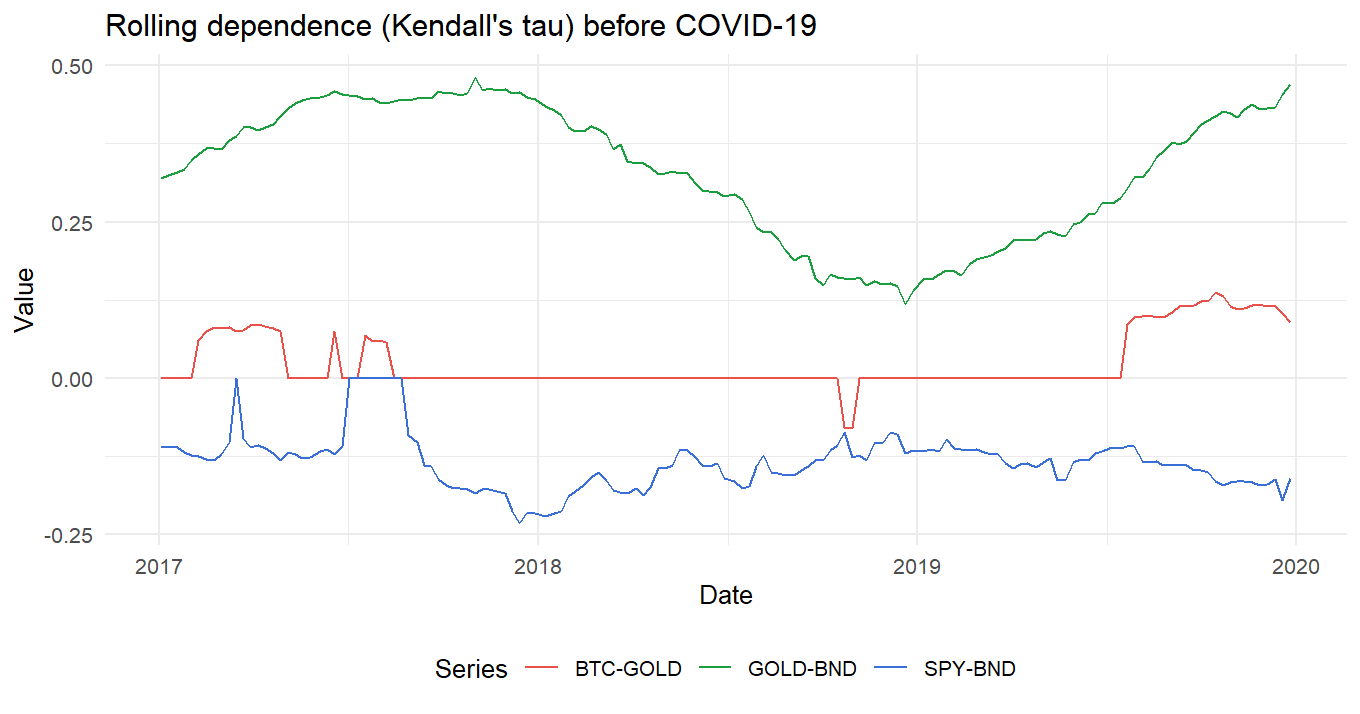
\includegraphics[width=0.85\textwidth]{figures/report_pre_tau.png}
\caption{Rolling Kendall's $\tau$ before COVID-19}
\end{figure}
\begin{itemize}
  \item GOLD--BND. Kendall's $\tau$ is above 0.4 in 2017, falls to roughly 0.12 between late 2018 and early 2019, then rises to around 0.4 by the end of 2019. The positive association is consistent with the behavior of gold and bonds under low interest rates.
  \item SPY--BND. Dependence remains nonpositive, with $\tau$ between 0 and $-0.23$. The negative relationship stabilizes from 2018, consistent with bonds hedging equities.
  \item BTC--GOLD. Dependence stays near zero ($-0.08$ to 0.14), and the independence test usually does not reject. The relationship becomes weakly positive at the end of 2019 ($\tau\approx0.10$).
\end{itemize}

The LTD curve tracks dependence in joint extreme declines.
\begin{figure}[H]
\centering
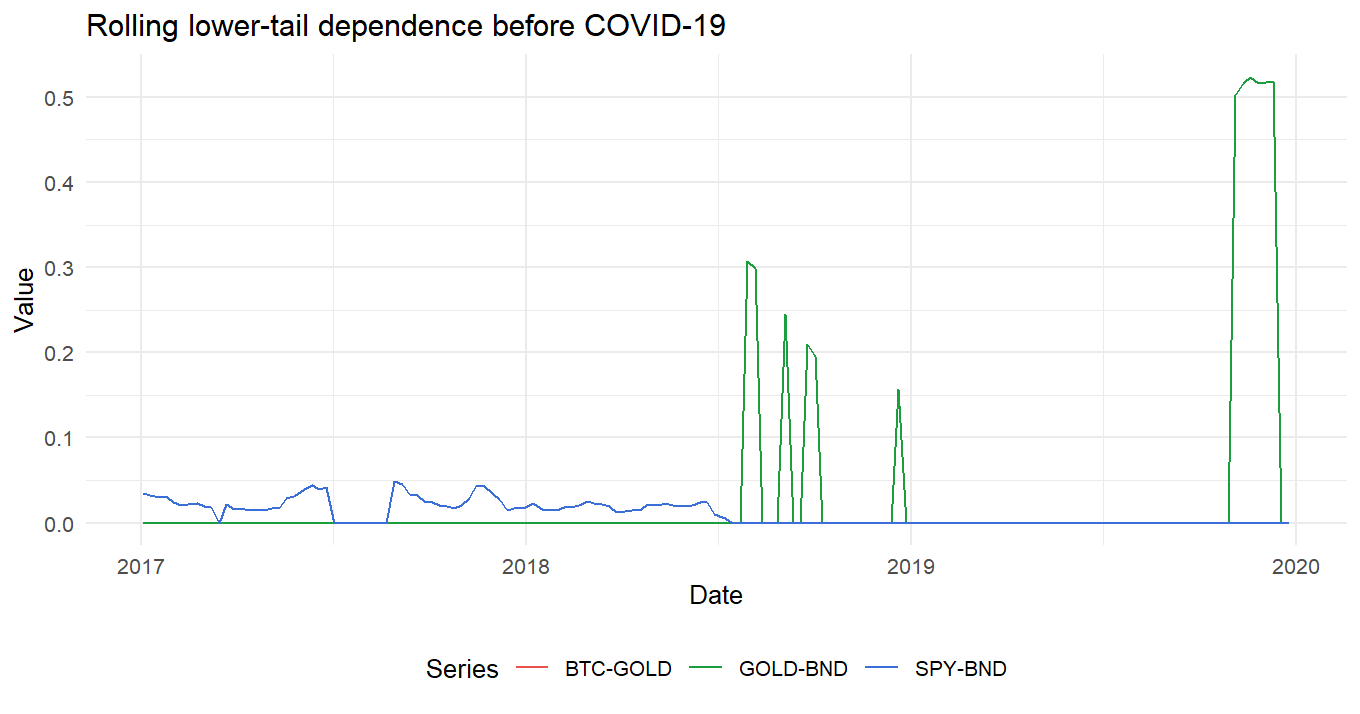
\includegraphics[width=0.85\textwidth]{figures/report_pre_LTD.png}
\caption{Rolling lower-tail dependence before COVID-19}
\end{figure}
\begin{itemize}
  \item GOLD--BND. LTD is zero in 92\% of windows, with occasional values around 0.2 to 0.3 in 2018--2019 and a peak of 0.52 in November 2019. The two safe havens can experience sharp joint declines during some bond market or liquidity shocks.
  \item BTC--GOLD. LTD is zero throughout the period.
  \item SPY--BND. LTD remains below 0.05, consistent with bonds providing some protection against extreme equity losses before COVID-19.
\end{itemize}

The UTD curve tracks dependence in joint extreme gains.
\begin{figure}[H]
\centering
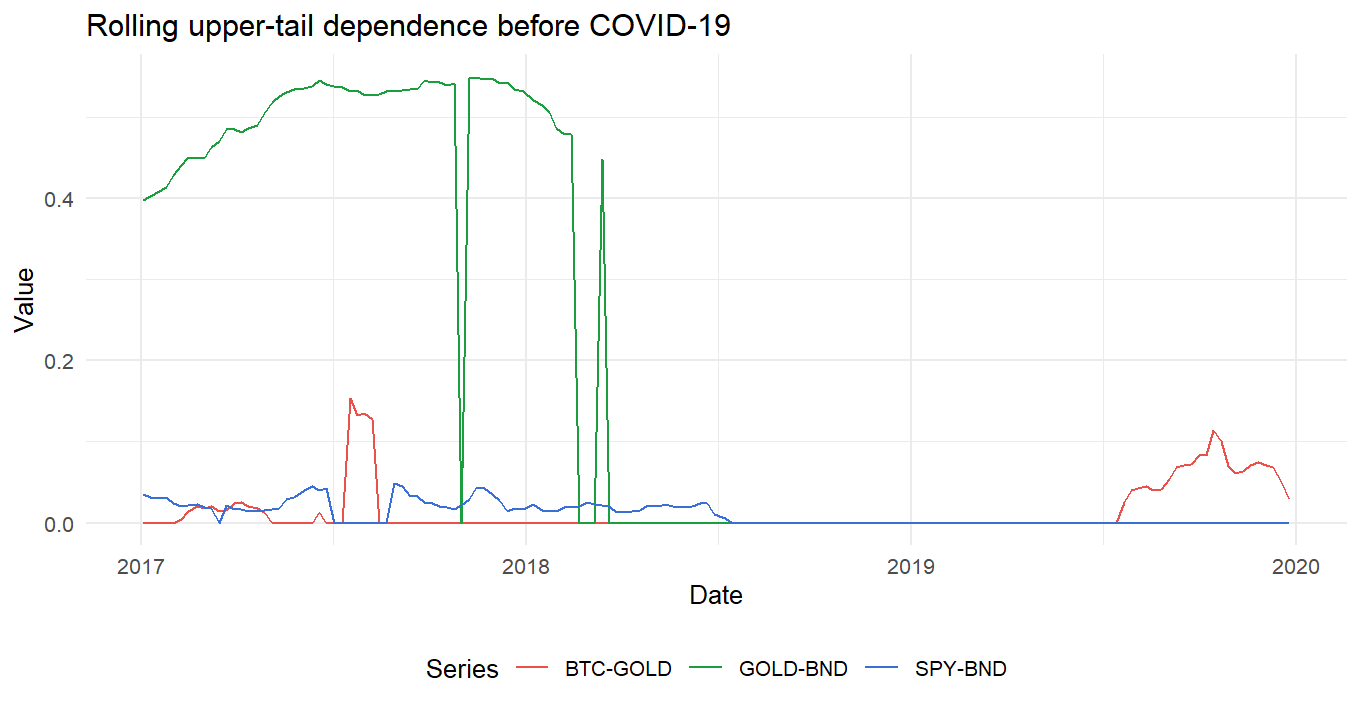
\includegraphics[width=0.85\textwidth]{figures/report_pre_UTD.png}
\caption{Rolling upper-tail dependence before COVID-19}
\end{figure}
\begin{itemize}
  \item GOLD--BND. UTD is around 0.5 to 0.55 early in the period and falls substantially after 2018. Early joint gains may reflect demand for safety or changing expectations about monetary policy.
  \item BTC--GOLD. UTD is zero in 74\% of windows and peaks at 0.15 in summer 2017. Extreme gains in Bitcoin and gold remain largely separate.
  \item SPY--BND. UTD is low and often close to zero.
\end{itemize}

\paragraph{Rolling dependence during COVID-19}
The rolling results show how diversification relationships changed in 2020 and 2021.
\begin{figure}[H]
\centering
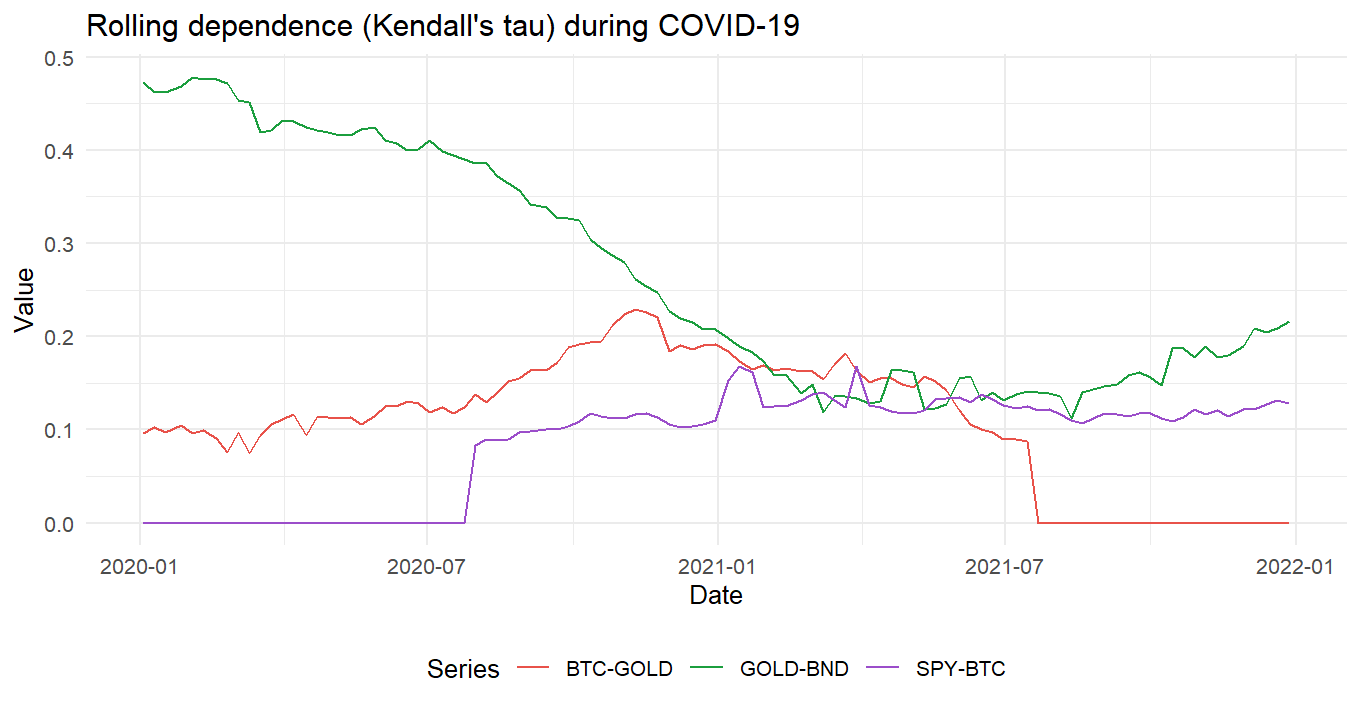
\includegraphics[width=0.85\textwidth]{figures/report_cov_tau.png}
\caption{Rolling Kendall's $\tau$ during COVID-19}
\end{figure}
\begin{itemize}
  \item SPY--BTC. Kendall's $\tau$ is zero in the first half of 2020, turns positive from summer 2020, and ranges from 0.10 to 0.17 in 2021. This is consistent with Bitcoin's increasing association with equities and the full-period estimate of 0.13.
  \item BTC--GOLD. Dependence peaks near 0.23 in early 2021 and drops to near zero in the second half of 2021. Bitcoin and gold became less closely linked after the early recovery.
  \item GOLD--BND. Kendall's $\tau$ starts near 0.44 in the first half of 2020 and falls to around 0.15 in 2021.
\end{itemize}

The LTD curves show how the risk of joint extreme losses evolved.
\begin{figure}[H]
\centering
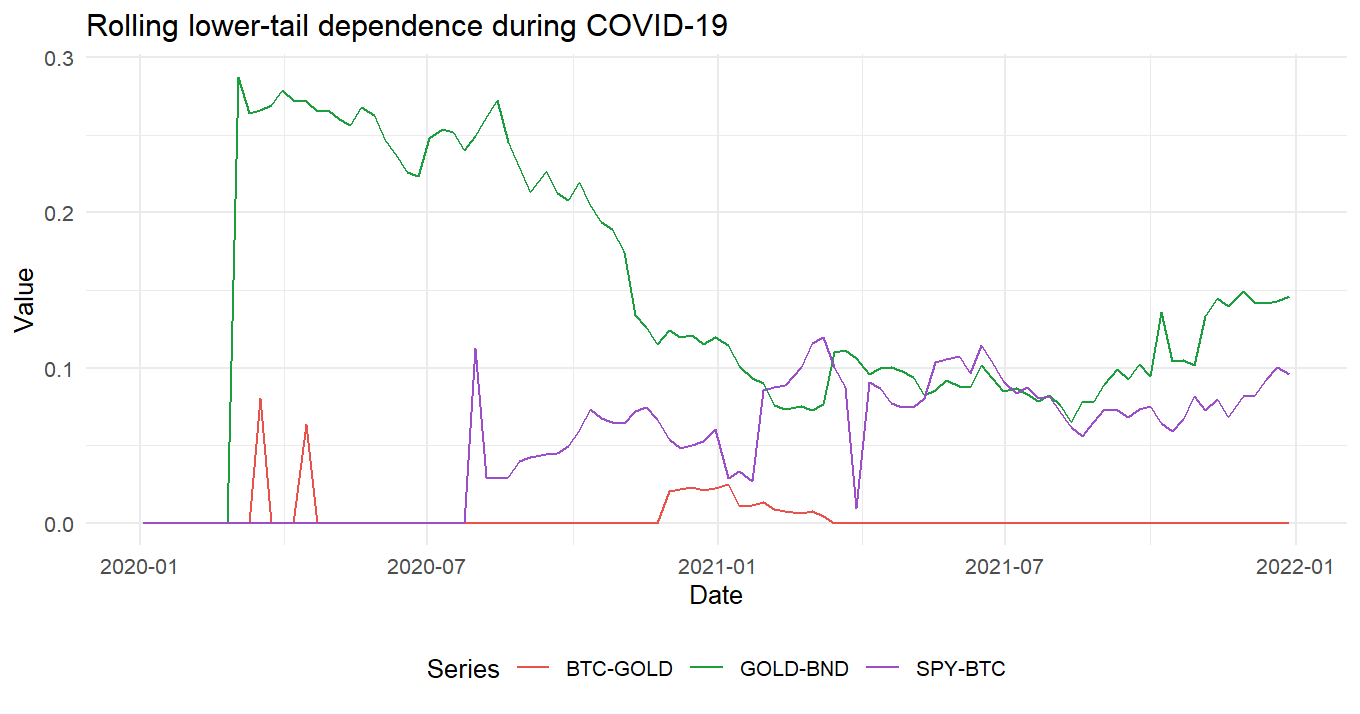
\includegraphics[width=0.85\textwidth]{figures/report_cov_LTD.png}
\caption{Rolling lower-tail dependence during COVID-19}
\end{figure}
\begin{itemize}
  \item SPY--BTC. LTD is zero until summer 2020, then ranges from 0.03 to 0.12, peaking in March 2021. This is consistent with the Clayton copula selected for the full crisis period.
  \item GOLD--BND. LTD reaches 0.29 in March 2020, stays above 0.20 until autumn 2020, and falls toward 0.10 in 2021. The rise in joint declines among safe-haven assets is consistent with a broad move toward cash.
  \item BTC--GOLD. LTD peaks at 0.08 in March 2020 but is zero in 84\% of windows. Joint extreme declines appear episodic, consistent with the zero LTD of the fitted BB7 copula.
\end{itemize}

The UTD curves track joint extreme gains during the crisis.
\begin{figure}[H]
\centering
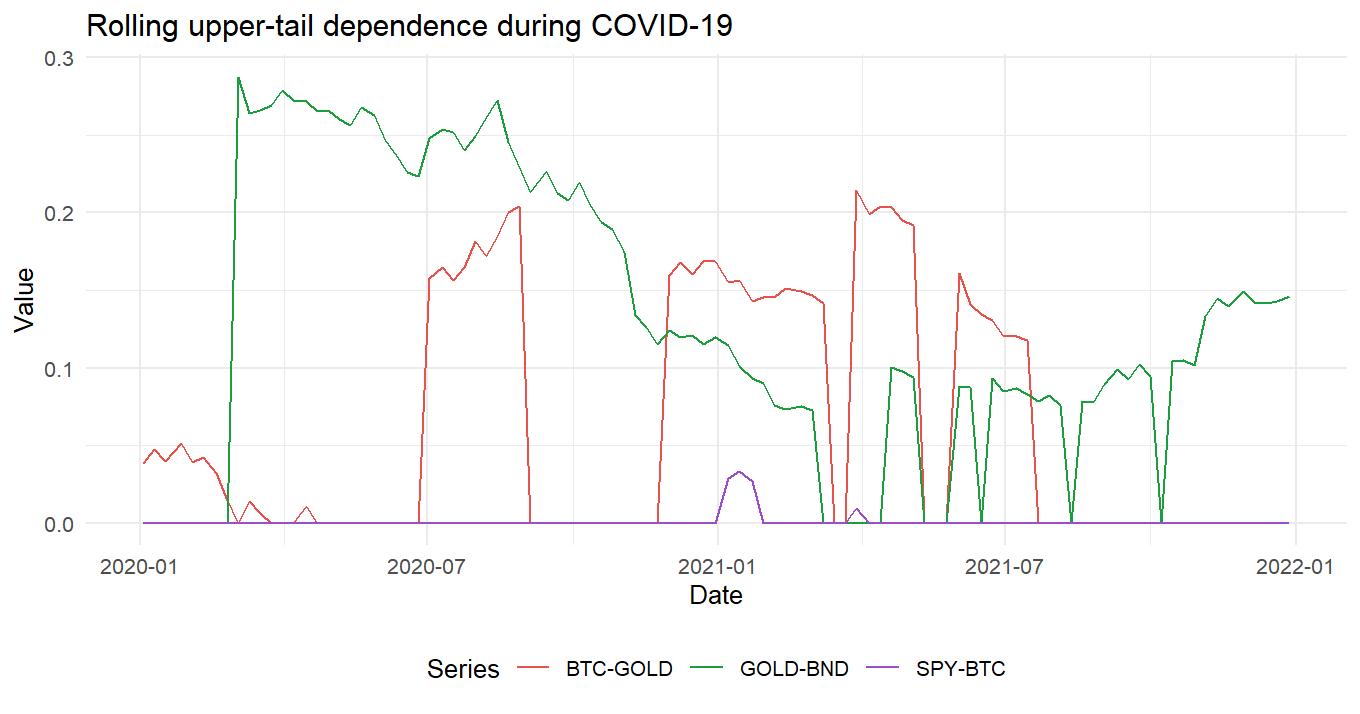
\includegraphics[width=0.85\textwidth]{figures/report_cov_UTD.png}
\caption{Rolling upper-tail dependence during COVID-19}
\end{figure}
\begin{itemize}
  \item BTC--GOLD. UTD peaks at 0.21 in March 2021, compared with a full-period estimate of 0.10. Joint gains may reflect periods when investors treated Bitcoin as a hedge against inflation.
  \item SPY--BTC. UTD is zero in 96\% of windows and peaks at 0.03. Crisis dependence is concentrated in the lower tail.
  \item GOLD--BND. UTD is around 0.18 in 2020, with a maximum of 0.29 in March, and ranges from 0.05 to 0.10 in 2021.
\end{itemize}
Lower-tail dependence between gold and bonds strengthened during the COVID-19 crisis. Bitcoin and equities also showed a moderate risk of joint sharp declines. Joint extreme gains among Bitcoin, equities, and gold remained limited.

\paragraph{Post-COVID rolling dependence}
From 2022 through 2025, dependence stabilized under a new market regime characterized by persistent inflation and shifts in monetary policy.

Dependence became more stable and symmetric, and generally stronger than before COVID-19.
\begin{figure}[H]
\centering
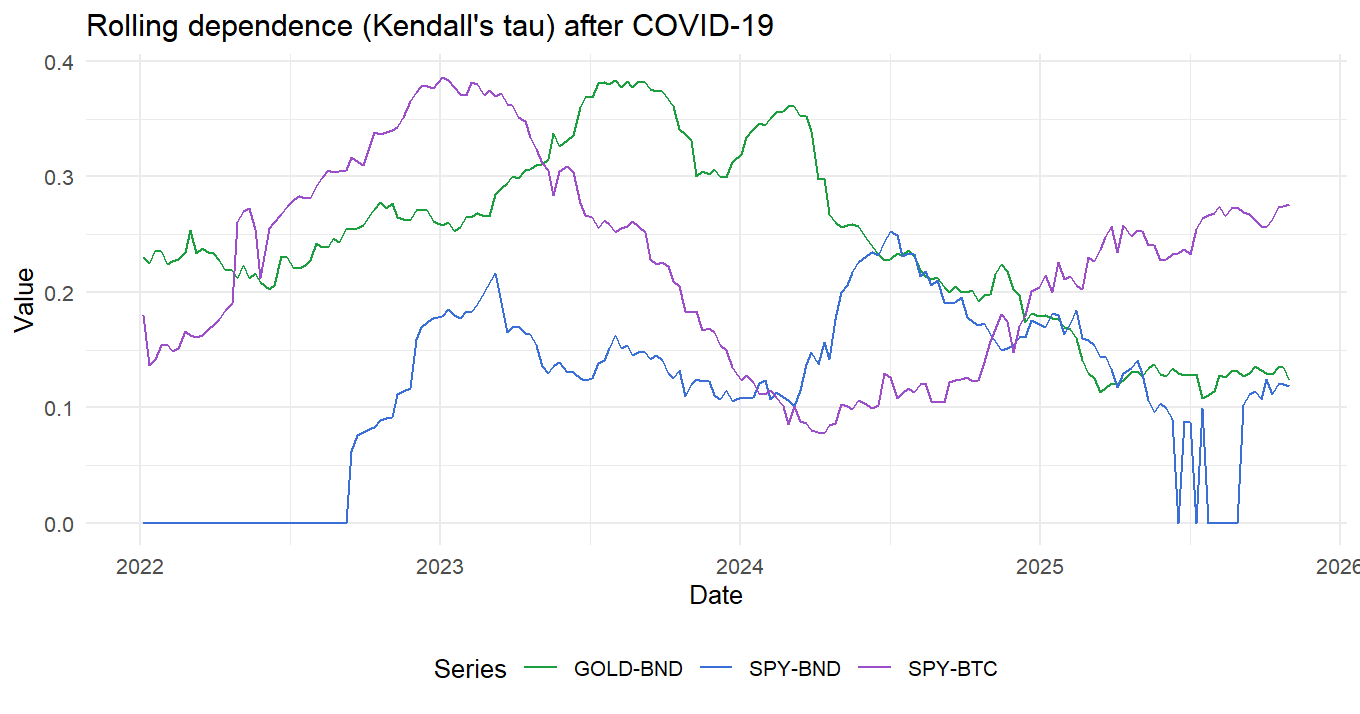
\includegraphics[width=0.85\textwidth]{figures/report_post_tau.png}
\caption{Rolling Kendall's $\tau$ after COVID-19}
\end{figure}
\begin{itemize}
  \item SPY--BTC. Kendall's $\tau$ ranges from 0.08 to 0.39. Six-month averages range from 0.20 to 0.34 in 2022--2023, dip to about 0.10 in the first half of 2024, and recover to around 0.25 in 2025. The positive relationship indicates stronger integration of Bitcoin with equities.
  \item GOLD--BND. Dependence has generally declined since 2024, from around 0.35 at the end of 2023 to 0.13 in 2025, below the stronger levels observed before COVID-19.
  \item BND--SPY. Dependence is still near zero in early 2022, then is predominantly positive, ranging from 0.10 to 0.25 from 2023. The shift from stable negative dependence before COVID-19 is consistent with weaker bond hedging under inflationary pressure.
\end{itemize}

The UTD curves show how joint extreme gains evolve after the crisis.
\begin{figure}[H]
\centering
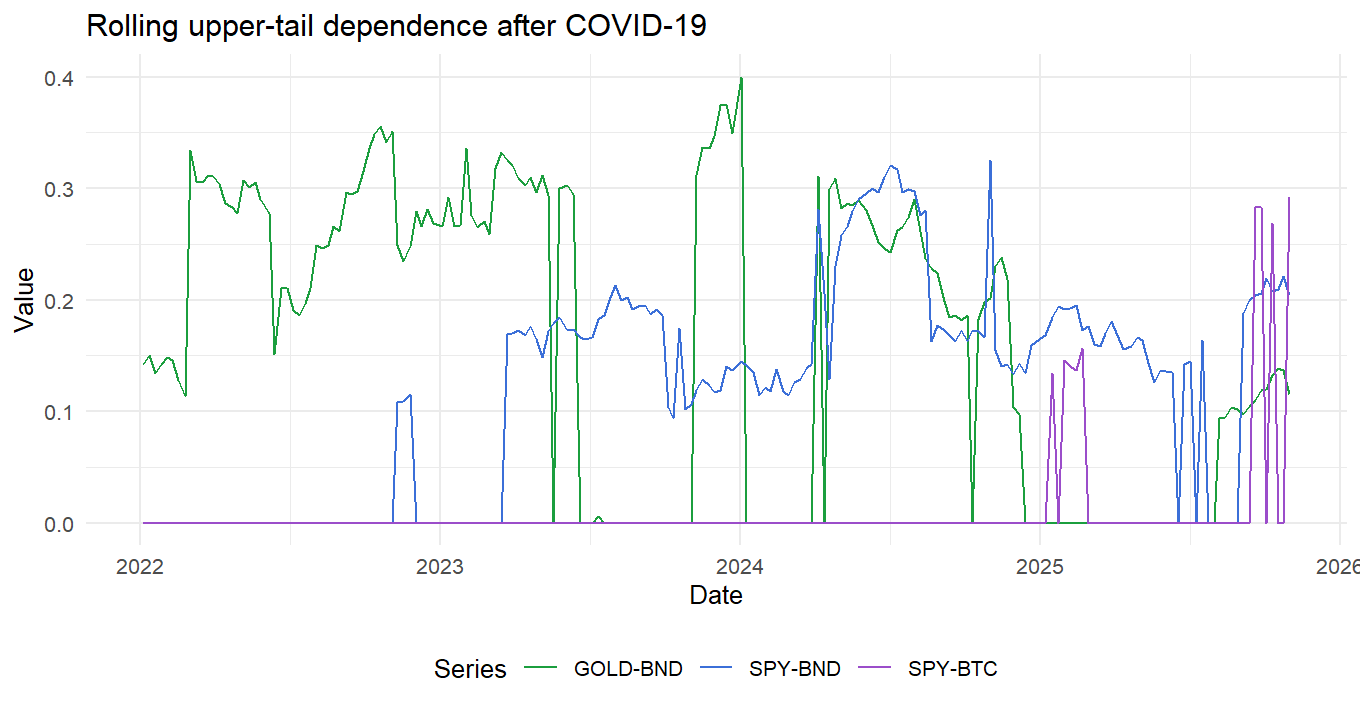
\includegraphics[width=0.85\textwidth]{figures/report_post_UTD.png}
\caption{Rolling upper-tail dependence after COVID-19}
\end{figure}
\begin{itemize}
  \item SPY--BTC. UTD is zero in 95\% of windows and rises to 0.29 in late 2025.
  \item BND--SPY. UTD becomes moderate from 2023, generally ranging from 0.10 to 0.20, with a maximum of 0.33 in late 2024. Equities and bonds can rally together as rates ease.
  \item GOLD--BND. UTD weakens after 2024 toward 0.10--0.20, with an earlier peak of 0.40 in early 2024.
\end{itemize}

The final figure shows rolling lower-tail dependence from 2022 to 2025.
\begin{figure}[H]
\centering
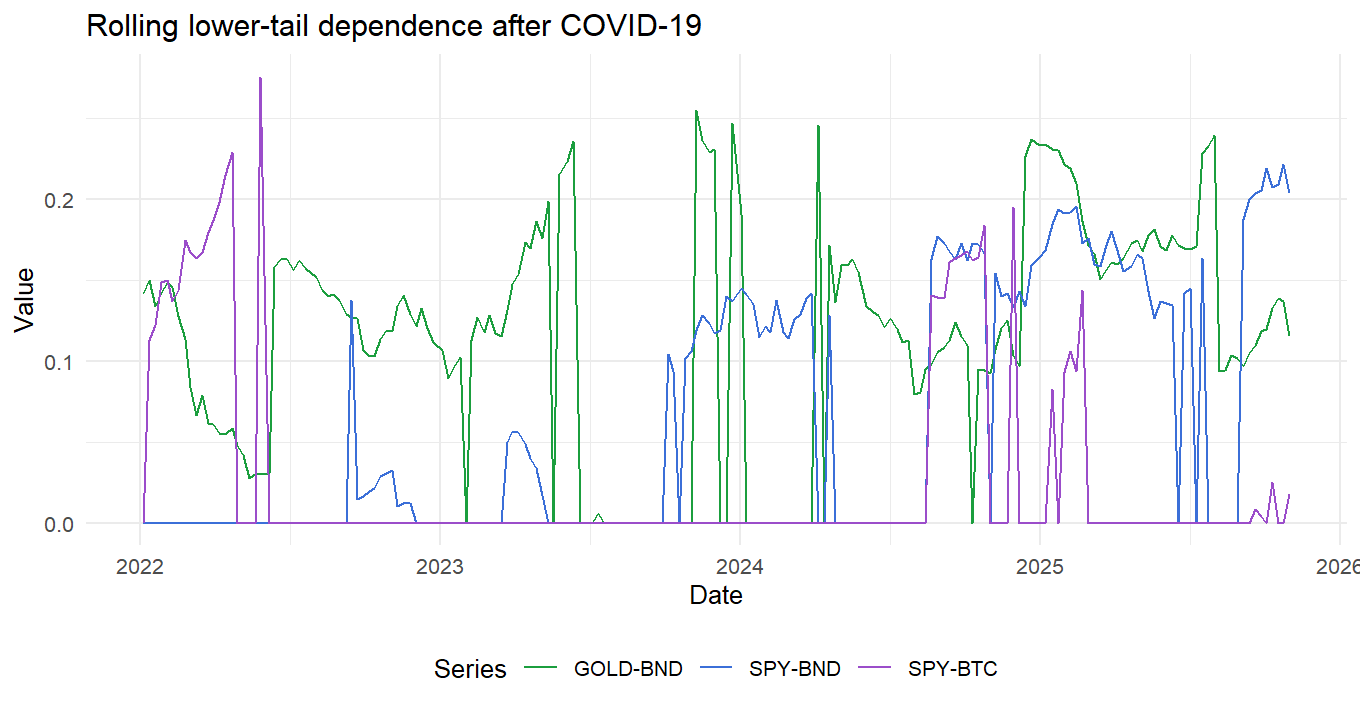
\includegraphics[width=0.85\textwidth]{figures/report_post_LTD.png}
\caption{Rolling lower-tail dependence after COVID-19}
\end{figure}
\begin{itemize}
  \item BND--SPY. LTD rises from near zero in 2022 to around 0.07--0.16 in 2024--2025, with a peak of 0.22 in October 2025. These episodes reflect joint equity and bond declines, possibly during inflation or monetary tightening shocks.
  \item GOLD--BND. LTD is moderate and persistent, with six-month averages of 0.05--0.18. It is zero in only 19\% of windows and reaches 0.26 in November 2023.
  \item SPY--BTC. LTD is zero in 81\% of windows. It peaks at 0.28 in May 2022 during the Terra-Luna collapse, reappears around 0.07 in the second half of 2024, and stays near zero in 2025.
  \item Bitcoin's increasing integration is clearer in Kendall's $\tau$ (around 0.25 in 2025) than in the frequency of joint crashes. The introduction of spot Bitcoin ETFs and institutional portfolio adoption may help explain this change.
\end{itemize}

% =====================================================================================================
\section{Portfolio Optimization Results}\label{sec:allocation}
\begin{correction}

We compare six allocation strategies from November 2019 to November 2025. Two minimize variance or CVaR using historical returns. Two use scenarios simulated from the ARMA-EGARCH R-vine. We also include the equally weighted portfolio (1/N) and a minimum-CVaR strategy that uses the same ARMA-EGARCH margins with a Gaussian copula. Short selling is prohibited, asset weights are capped at 50\%, and the risk-free rate is set to 2\%.

\subsection{Backtest Design}

Portfolios are rebalanced every five trading sessions, for 302 rebalances between November 4, 2019 and November 3, 2025. At each rebalance, \texttt{rugarch} estimates the ARMA-EGARCH margins with standardized Student-t innovations using up to 1,000 prior daily returns. The copula is fitted to the last 504 pseudo-observations. We simulate next-day returns as
\[
r_{i,t+1} = \hat\mu_{i,t+1} + \hat\sigma_{i,t+1}\,(F^{\mathrm{std}}_{\nu_i})^{-1}(U_i),
\]
where \(U_i\) is the simulated uniform component for asset \(i\).

We use 10,000 scenarios per draw and five random seeds for the simulated CVaR strategies. The simulated minimum-variance strategy uses the first draw. We minimize 95\% CVaR using the formulation of \citet{rockafellar2000}. The historical strategies use the most recent 252 observed returns. Transaction costs are 10 basis points per unit of turnover, and weights drift with prices between rebalances.

\subsection{Strategy Performance}

\begin{table}[H]
\centering
\resizebox{\textwidth}{!}{%
\begin{tabular}{lrrrrrrrrr}
\toprule
Strategy & Total return & Ann. return & Ann. vol. & Sharpe & Sortino & Max DD & Calmar & Daily CVaR & Turnover \\
 & (\%) & (\%) & (\%) & & & (\%) & & 95\% (\%) & /year \\
\midrule
Equal weight (1/N) & 278.09 & 24.89 & 19.25 & 1.189 & 1.705 & -34.70 & 0.717 & 2.68 & 1.4 \\
Historical MinVar & 55.73 & 7.68 & 8.61 & 0.660 & 0.920 & -16.66 & 0.461 & 1.23 & 0.8 \\
Historical MinCVaR & 54.59 & 7.55 & 8.66 & 0.641 & 0.891 & -17.04 & 0.443 & 1.24 & 1.1 \\
MinVar R-vine ARMA-EGARCH & 65.90 & 8.83 & 8.19 & 0.834 & 1.172 & -15.62 & 0.565 & 1.16 & 6.3 \\
MinCVaR R-vine ARMA-EGARCH & 66.95 & 8.94 & 8.23 & 0.844 & 1.185 & -15.74 & 0.568 & 1.16 & 6.2 \\
Gaussian copula MinCVaR & 66.13 & 8.85 & 8.13 & 0.843 & 1.188 & -15.60 & 0.568 & 1.15 & 5.9 \\
\bottomrule
\end{tabular}}
\caption{Out-of-sample strategy performance, net of transaction costs}
\label{tab:perf}
\end{table}

The ARMA-EGARCH R-vine CVaR strategy earns a total return of 66.95\%, compared with 55.73\% for historical minimum variance. Their Sharpe ratios are 0.844 and 0.660, respectively. With the same margins, Gaussian copula CVaR achieves a Sharpe ratio of 0.843. The equally weighted portfolio earns 278.09\% in total and records a maximum drawdown of $-34.70\%$.

\subsection{Performance and Portfolio Weights Over Time}

Figure~\ref{fig:relative} shows cumulative wealth relative to the historical minimum-variance benchmark. From February 20 to March 23, 2020, the ARMA-EGARCH R-vine CVaR strategy returns $-8.83\%$, compared with $-9.62\%$ for historical minimum variance and $-7.82\%$ for Gaussian copula CVaR.

\begin{figure}[H]
\centering
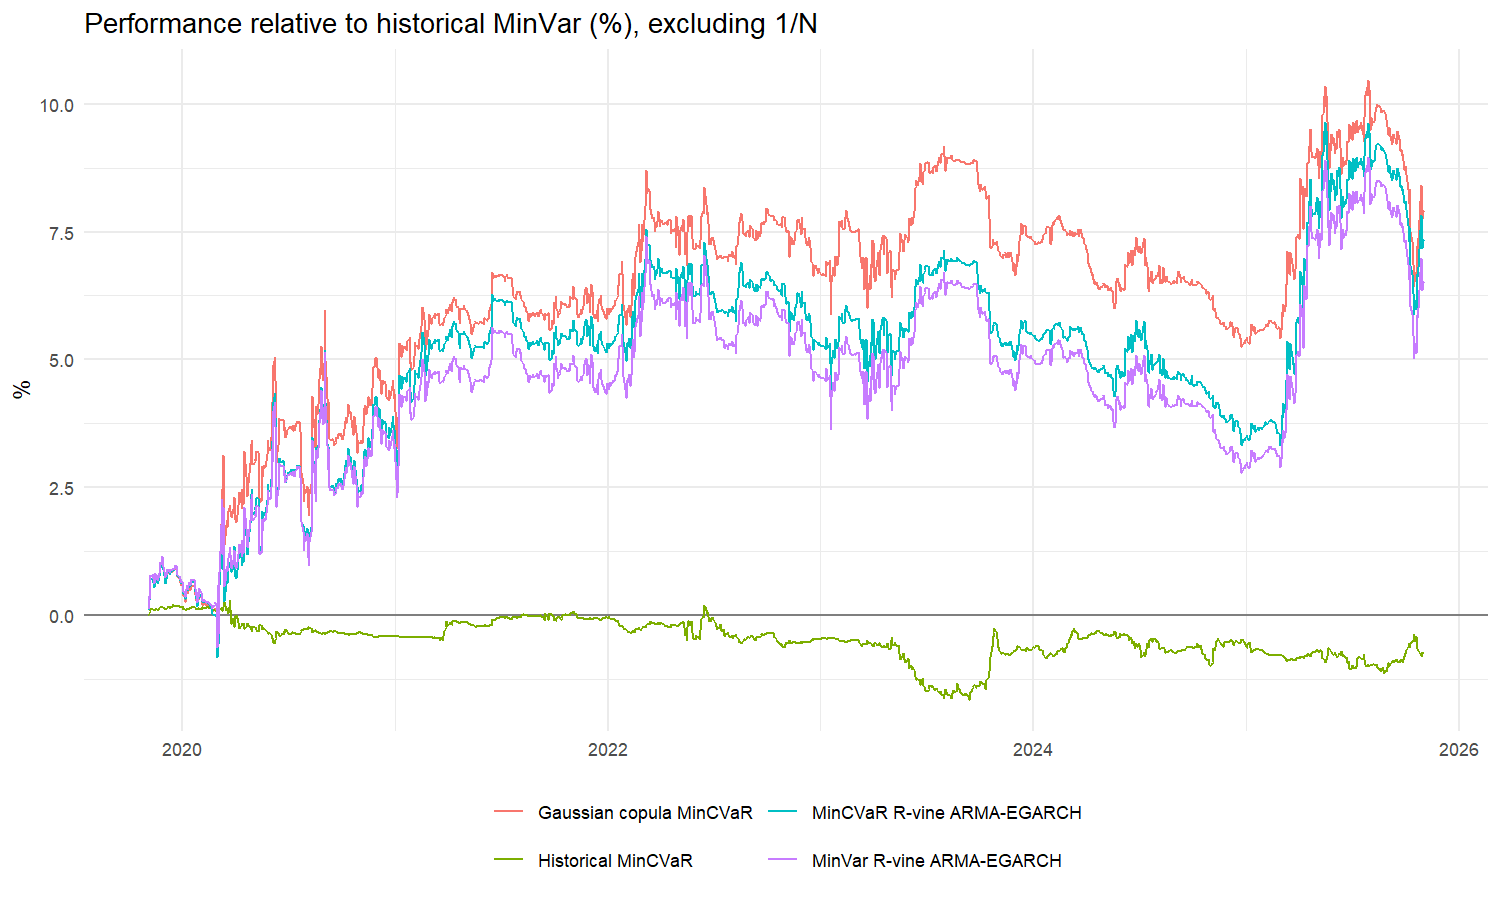
\includegraphics[width=0.95\textwidth]{figures/04_relative_performance.png}
\caption{Performance relative to historical minimum variance, excluding the equally weighted portfolio}
\label{fig:relative}
\end{figure}

Figure~\ref{fig:weights} shows the weekly weights for the first ARMA-EGARCH R-vine CVaR draw. On average, the portfolio allocates 49.9\% to BND, 28.2\% to SPY, 21.6\% to gold, and 0.3\% to Bitcoin. The small Bitcoin allocation limits the influence of its tail dependence on the portfolio.

\begin{figure}[H]
\centering
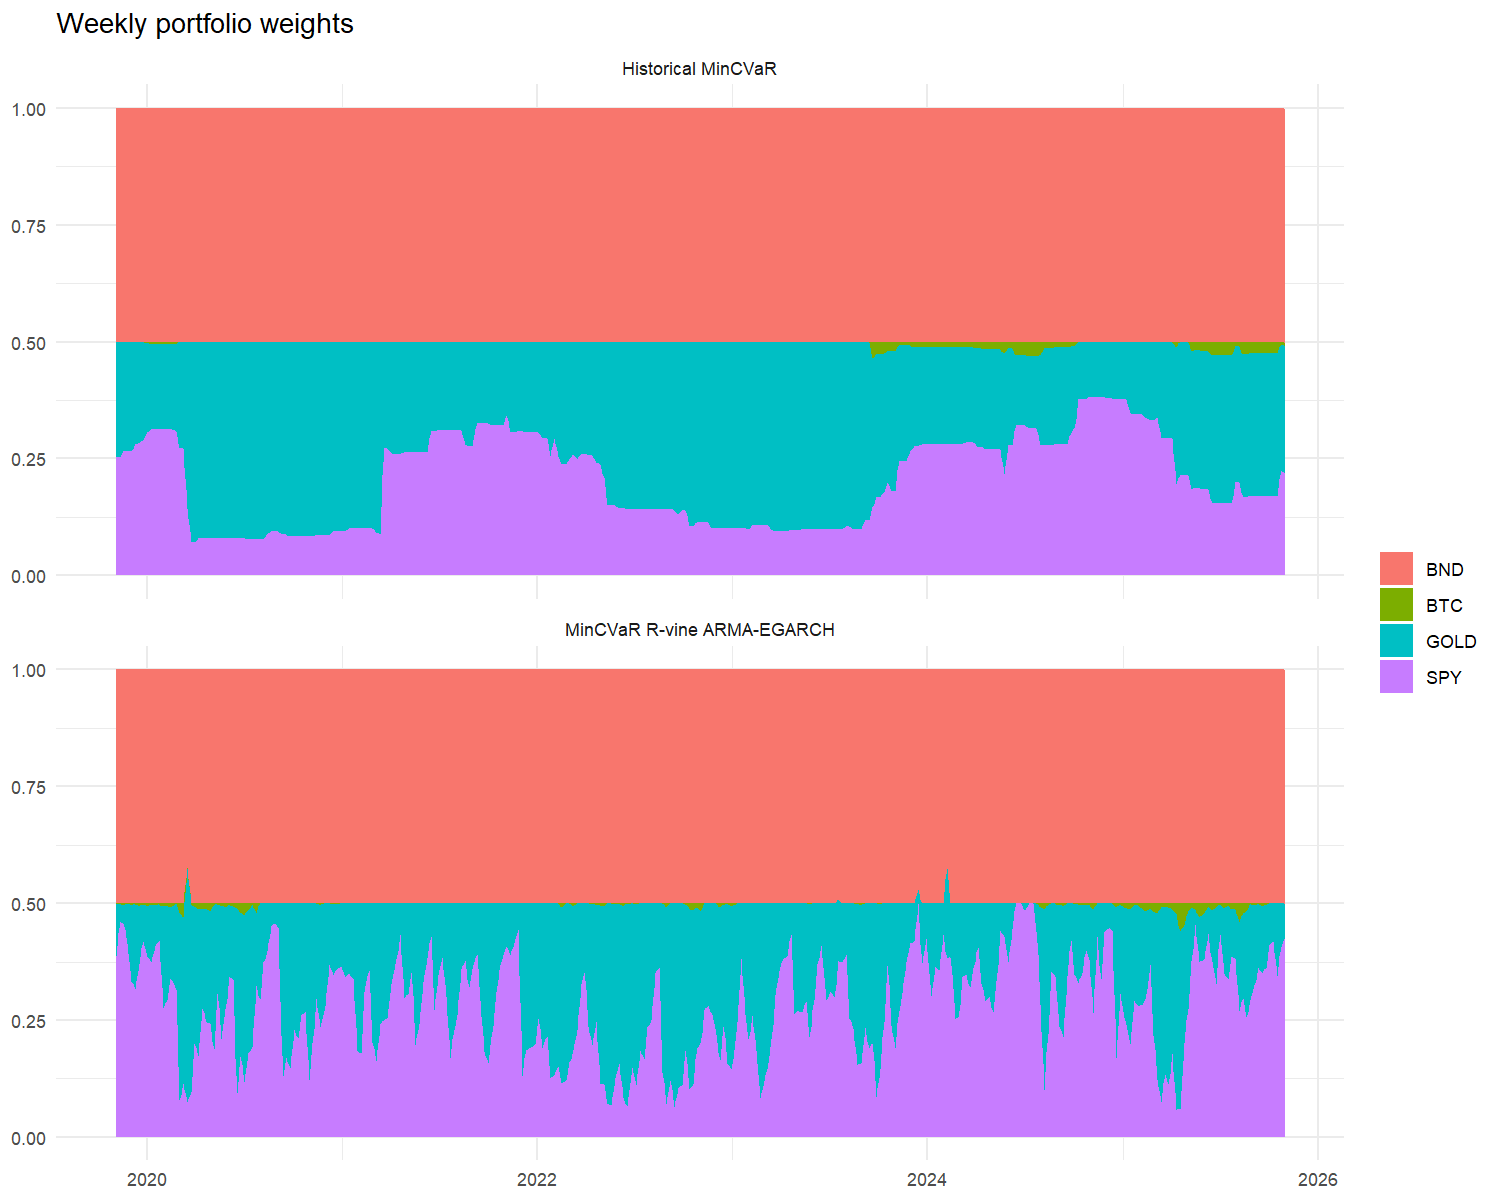
\includegraphics[width=0.95\textwidth]{figures/05_weights.png}
\caption{Weekly weights for ARMA-EGARCH R-vine CVaR and historical CVaR portfolios}
\label{fig:weights}
\end{figure}

\subsection{Statistical Significance and Monte Carlo Variation}\label{sec:monte-carlo}

We assess performance differences with a circular block bootstrap \citep{politis1992} on paired daily returns. We use 2,000 replications and blocks of 20 trading sessions. The comparisons use the first random seed.

\begin{table}[H]
\centering
\resizebox{\textwidth}{!}{%
\begin{tabular}{lrrrrrr}
\toprule
Comparison strategy & $\Delta$ Sharpe & p-value & $\Delta$ CVaR (pp) & p-value & $\Delta$ Max DD (pp) & p-value \\
\midrule
Equal weight (1/N) & -0.343 & 0.433 & -1.510 & 0.000 & 18.885 & 0.004 \\
Historical MinVar & 0.186 & 0.179 & -0.063 & 0.147 & 0.842 & 0.573 \\
Historical MinCVaR & 0.204 & 0.182 & -0.075 & 0.112 & 1.227 & 0.406 \\
MinVar R-vine ARMA-EGARCH & 0.011 & 0.564 & 0.007 & 0.222 & -0.190 & 0.402 \\
Gaussian copula MinCVaR & -0.031 & 0.386 & 0.026 & 0.093 & -0.464 & 0.441 \\
\bottomrule
\end{tabular}}
\caption{Performance differences between ARMA-EGARCH R-vine CVaR and the comparison strategies}
\end{table}

The Sharpe comparison with historical minimum variance gives a p-value of 0.179. The comparison with Gaussian copula CVaR gives a p-value of 0.386. Neither difference is statistically significant at the 5\% level.

\begin{table}[H]
\centering
\resizebox{\textwidth}{!}{%
\begin{tabular}{lrrrr}
\toprule
Strategy & Scenarios & Sharpe & Total return (\%) & Max DD (\%) \\
\midrule
MinCVaR R-vine ARMA-EGARCH & 10\,000 & 0.827 -- 0.865 & 65.78 -- 68.30 & -15.92 -- -15.51 \\
MinCVaR R-vine ARMA-EGARCH & 500 & 0.795 -- 0.937 & 62.85 -- 74.08 & -16.34 -- -15.43 \\
Gaussian copula MinCVaR & 10\,000 & 0.800 -- 0.877 & 63.25 -- 68.07 & -15.93 -- -15.27 \\
\bottomrule
\end{tabular}}
\caption{Minimum and maximum across five random seeds}
\label{tab:mc}
\end{table}

For ARMA-EGARCH R-vine CVaR, Sharpe ranges from 0.795 to 0.937 with 500 scenarios and from 0.827 to 0.865 with 10,000. The ranges show how sensitive the results are to the number of scenarios.

\subsection{Value at Risk and Expected Shortfall Backtests}

For the equally weighted portfolio, we forecast 95\% and 99\% VaR and 97.5\% Expected Shortfall over 1,508 trading sessions. Model parameters are re-estimated weekly, and conditional volatility is updated daily. We use the VaR tests of \citet{kupiec1995} and \citet{christoffersen1998} and the ES test of \citet{mcneil2000}.

\begin{table}[H]
\centering
\resizebox{\textwidth}{!}{%
\begin{tabular}{lrrrrrrr}
\toprule
Model & Exceed. & Kupiec p & Christ. p & Exceed. & Kupiec p & Christ. p & ES p \\
 & VaR 95\% & 95\% & 95\% & VaR 99\% & 99\% & 99\% & 97.5\% \\
\midrule
R-vine ARMA-EGARCH & 4.78 & 0.686 & 0.878 & 1.06 & 0.814 & 0.819 & 0.333 \\
EGARCH + Gaussian copula & 4.78 & 0.686 & 0.878 & 1.06 & 0.814 & 0.819 & 0.264 \\
EGARCH + independence & 6.50 & 0.011 & 0.021 & 1.26 & 0.329 & 0.488 & 0.692 \\
Historical simulation (252 days) & 4.58 & 0.443 & 0.665 & 1.33 & 0.225 & 0.366 & 0.168 \\
Normal variance-covariance (252 days) & 4.04 & 0.079 & 0.137 & 1.33 & 0.225 & 0.366 & 0.022 \\
\bottomrule
\end{tabular}}
\caption{VaR and ES backtests for the equally weighted portfolio}
\label{tab:var}
\end{table}

The ARMA-EGARCH R-vine and Gaussian copula models both record exceedance rates of 4.78\% and 1.06\%, compared with expected rates of 5\% and 1\%. With independence, the 95\% VaR exceedance rate rises to 6.50\% (Kupiec p-value 0.011). The ES test gives p-values of 0.333 for the R-vine and 0.264 for the Gaussian copula. At the 5\% level, the VaR coverage and ES tests do not reject either model.

\begin{figure}[H]
\centering
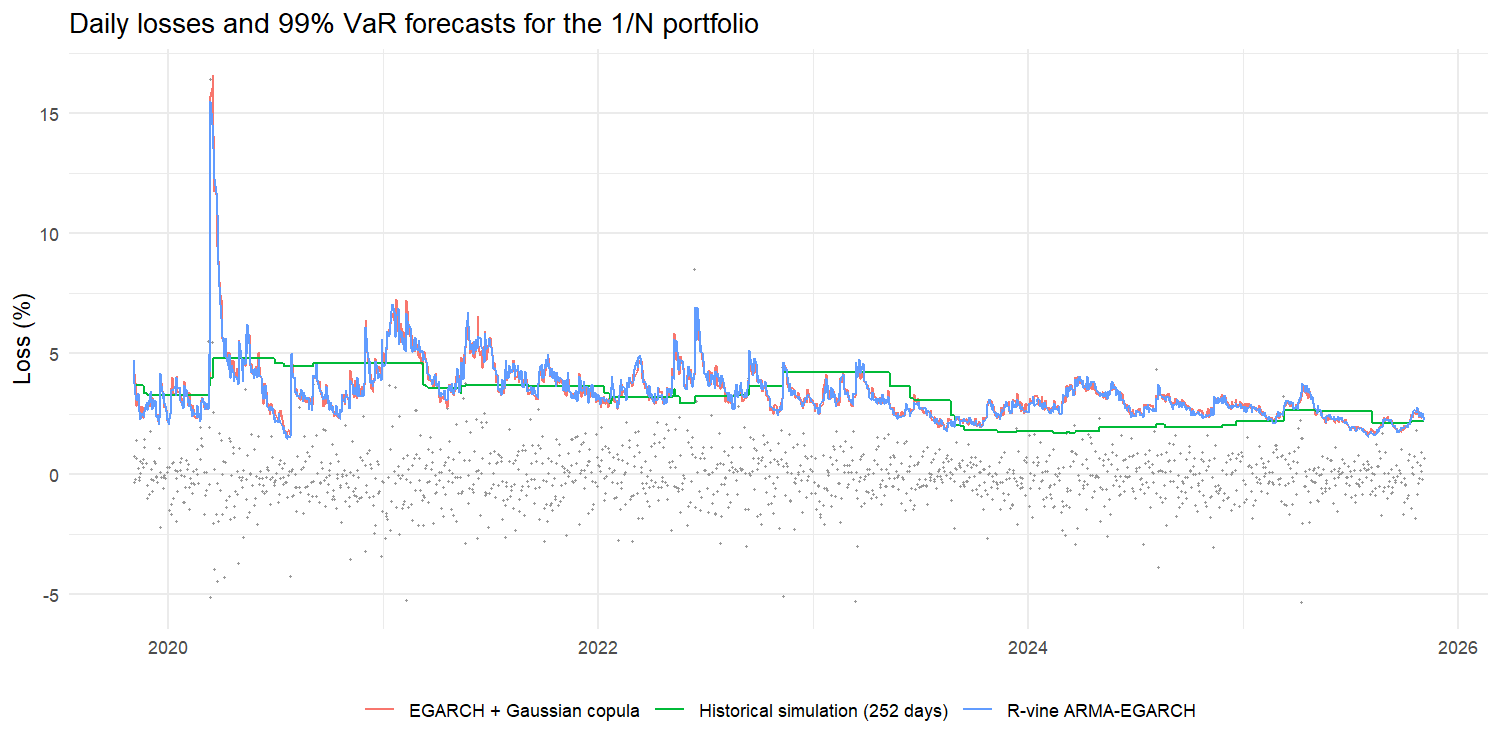
\includegraphics[width=0.95\textwidth]{figures/06_var99.png}
\caption{Daily losses and 99\% VaR forecasts for the equally weighted portfolio}
\end{figure}

\subsection{Practical Implications}

The ARMA-EGARCH R-vine CVaR strategy turns over 6.2 times the portfolio per year, compared with 0.8 for historical minimum variance. This difference matters when interpreting net performance. The similar results for the two copulas with identical margins should also be read in light of the observed weights, especially the small Bitcoin allocation.
\end{correction}

\section{Conclusion}

This study combines ARMA-GARCH models and vine copulas to quantify extreme dependence among US equities, Bitcoin, bonds, and gold from 2016 to 2025. The estimates identify a shift in the relationships among these assets and illustrate the limits of linear correlations for describing joint extremes during crises. Three findings stand out.

\begin{enumerate}
  \item Bitcoin shifts from near independence with gold and equities before 2020 to a closer relationship with equities afterward. Kendall's $\tau$ with SPY is 0.24 in the post-COVID period and around 0.25 in 2025, while lower-tail dependence is moderate (0.09 during the crisis and 0.12 afterward). The BND--SPY relationship shifts from negative before COVID ($\tau=-0.14$, LTD = 0.01) to positive afterward ($\tau=0.14$, UTD = LTD = 0.12), consistent with weaker bond hedging. In 2022, the minimum-risk strategies lose around 10\% as equities and bonds fall together. Gold and bonds remain positively dependent, with weaker tail dependence after 2022.
  \item The standardized Student-t distribution is used both to transform standardized residuals to uniforms and to simulate returns for risk measurement.
  \item The ARMA-EGARCH R-vine CVaR strategy achieves a Sharpe ratio of 0.844, versus 0.660 for historical minimum variance. With the same margins and a Gaussian copula, the Sharpe ratio is 0.843. The comparison between the two CVaR strategies gives a p-value of 0.386. The low weight of Bitcoin in minimum-risk portfolios limits the influence of its tail dependence.
\end{enumerate}

The framework extends conventional correlation-based analysis to multi-asset portfolios that include crypto-assets.

These results motivate further work on the use of tail dependence in allocation decisions.

Future work could examine how transaction costs affect the choice of recalibration frequency, broaden the asset universe, and develop conditional vine copulas with macroeconomic variables such as expected inflation, real rates, and the VIX. The latter extension would test whether the model can anticipate changes in dependence before episodes of stress.
Another extension would test portfolios with a material Bitcoin allocation, for example through a minimum-weight constraint or a return target, where asymmetric dependence may have a greater effect on the allocation.

% =====================================================================================================
\begin{correction}
\begin{thebibliography}{99}
\bibitem[Aas et~al.(2009)]{aas2009} Aas, K., Czado, C., Frigessi, A. and Bakken, H. (2009). ``Pair-copula constructions of multiple dependence''. In: \emph{Insurance: Mathematics and Economics} 44.2, pp.~182--198.
\bibitem[Bedford and Cooke(2002)]{bedford2002} Bedford, T. and Cooke, R. M. (2002). ``Vines -- a new graphical model for dependent random variables''. In: \emph{The Annals of Statistics} 30.4, pp.~1031--1068.
\bibitem[Christoffersen(1998)]{christoffersen1998} Christoffersen, P. F. (1998). ``Evaluating interval forecasts''. In: \emph{International Economic Review} 39.4, pp.~841--862.
\bibitem[Dissmann et~al.(2013)]{dissmann2013} Dissmann, J., Brechmann, E. C., Czado, C. and Kurowicka, D. (2013). ``Selecting and estimating regular vine copulae and application to financial returns''. In: \emph{Computational Statistics \& Data Analysis} 59, pp.~52--69.
\bibitem[Evkaya et~al.(2024)]{evkaya2024} Evkaya, O. et al. (2024). ``Vine copula approach to understand the financial dependence of the Istanbul stock exchange index''. In: \emph{Computational Economics} 64.5, pp.~2935--2980.
\bibitem[Ghalanos(n.d.)]{rugarch} Ghalanos, A. \emph{rugarch: Univariate GARCH models}. R package.
\bibitem[Kupiec(1995)]{kupiec1995} Kupiec, P. H. (1995). ``Techniques for verifying the accuracy of risk measurement models''. In: \emph{The Journal of Derivatives} 3.2, pp.~73--84.
\bibitem[McNeil and Frey(2000)]{mcneil2000} McNeil, A. J. and Frey, R. (2000). ``Estimate of tail-related risk measures for heteroscedastic financial time series: an extreme value approach''. In: \emph{Journal of Empirical Finance} 7.3--4, pp.~271--300.
\bibitem[Nelson(1991)]{nelson1991} Nelson, D. B. (1991). ``Conditional heteroskedasticity in asset returns: A new approach''. In: \emph{Econometrica} 59.2, pp.~347--370.
\bibitem[Politis and Romano(1992)]{politis1992} Politis, D. N. and Romano, J. P. (1992). ``A circular block-resampling procedure for stationary data''. In: LePage, R. and Billard, L. (eds.), \emph{Exploring the Limits of Bootstrap}. Wiley, pp.~263--270.
\bibitem[Rockafellar and Uryasev(2000)]{rockafellar2000} Rockafellar, R. T. and Uryasev, S. (2000). ``Optimization of conditional value-at-risk''. In: \emph{Journal of Risk} 2.3, pp.~21--41.
\bibitem[Schepsmeier et~al.(n.d.)]{vinecopula} Schepsmeier, U. et al. \emph{VineCopula: Statistical inference of vine copulas}. R package.
\bibitem[Sklar(1959)]{sklar1959} Sklar, M. (1959). ``Fonctions de répartition à n dimensions et leurs marges''. In: \emph{Annales de l'ISUP}. Vol.~8. 3, pp.~229--231.
\end{thebibliography}
\end{correction}


\end{document}
